\newpage
\section*{Part 3. Project identification: approved Project Proposal}
\addcontentsline{toc}{section}{Part 3. Project identification: approved Project Proposal}
\markright{Part 3. Project Proposal}
This section contains the problem identification in the form of the complete approved Project Proposal, unchanged from the final approved version.
\newpage
%Fix the format for this section
\titleformat{\section}[frame]
{\fontsize{12pt}{14.4pt}\selectfont\bfseries} {} {5pt} {}%{\thesection\quad}
\titleformat{\subsection}[display]
{\fontsize{18pt}{21.6pt}\selectfont\bfseries} {} {5pt} {}%{\thesubsection\quad}
\titleformat{\subsubsection}[display]
{\fontsize{14pt}{16.8pt}\selectfont\bfseries} {} {5pt} {\thesubsubsection\quad}
\renewcommand\thesubsection{\arabic{subsection}.}
\renewcommand\thesubsubsection{\arabic{subsection}.\arabic{subsubsection}}
\rhead{Part 3. Project Proposal}

\begin{refsection}
%%
%%  Department of Electrical, Electronic and Computer Engineering.
%%  EPR400/2 Project Proposal - Section 1.
%%  Copyright (C) 2011-2017 University of Pretoria.
%%

\section{Problem statement}

\textbf{Motivation.}


\textbf{Context.}

\textbf{Technical challenge.}

\textbf{Limitations.}

\nocite{Haykin:Communication_Systems}

%% End of File.


%%
%%  Department of Electrical, Electronic and Computer Engineering.
%%  EPR400/2 Project Proposal - Section 2.
%%  Copyright (C) 2011-2017 University of Pretoria.
%%

\section{Project requirements}

\secunderline{ELO 3: Design part of the project}

\subsection{Mission requirements of the product}
The mission requirement of the product is
\subsection{Student tasks: design}

\vspace{1em}
\secunderline{ELO 4: Investigative part of the project}

\subsection{Research questions}

\subsection{Student tasks: experimental work}

\newpage 

%% End of File.



%%
%%  Department of Electrical, Electronic and Computer Engineering.
%%  EPR400/2 Project Proposal - Section 3.
%%  Copyright (C) 2011-2017 University of Pretoria.
%%

\section{Project plan}

This section includes the planning for the complete project period which spans over the period 1 February 2017 to 30 November 2017. The planning is in the form of a Gantt chart with a one week resolution. Figure \ref{fig:Gantt1} below shows the planning for the project up to the date of handing in this report. The blocks coloured in blue therefore represent work that is already completed.\\

\begin{figure}[htbp]
    \centering
        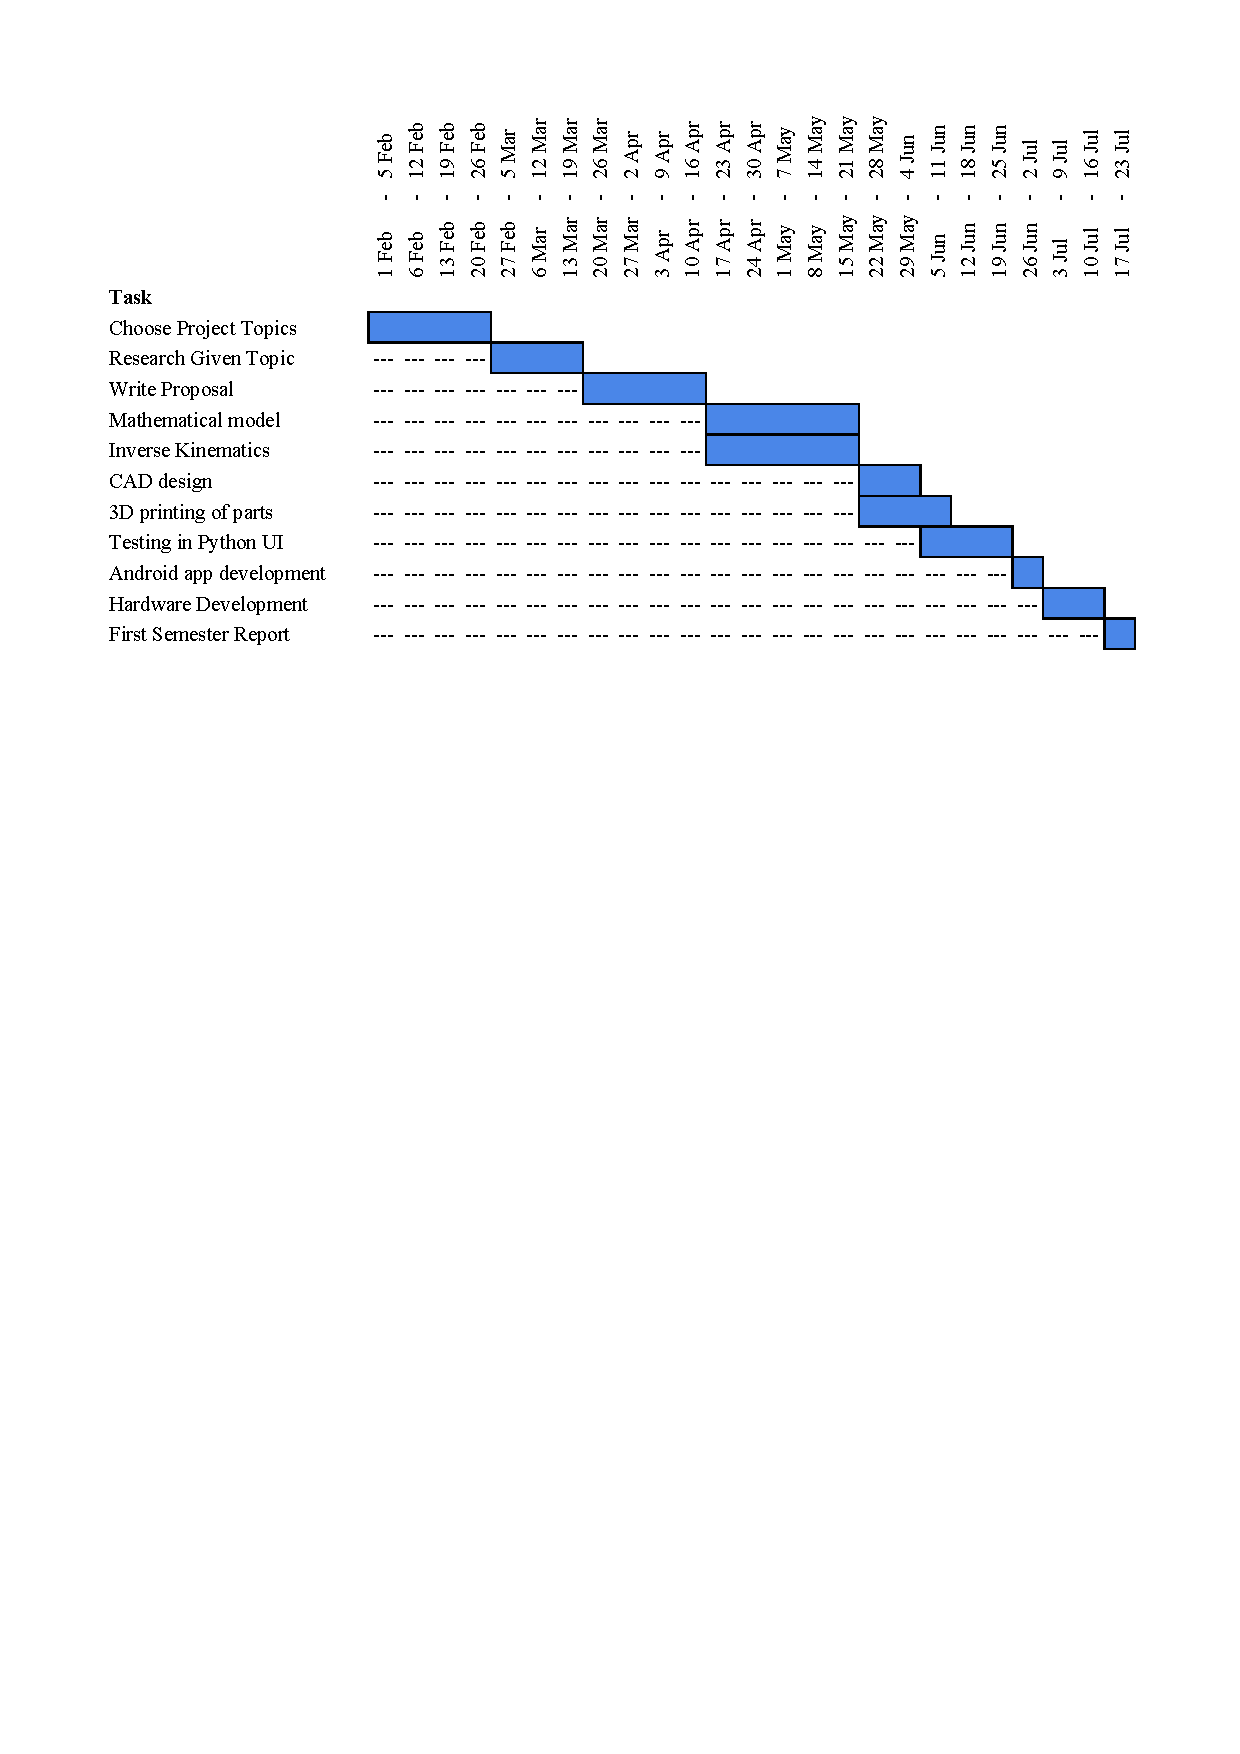
\includegraphics[clip, trim=1.5cm 18cm 1.5cm 1.5cm, width=1.00\textwidth]{pics/Gantt1.pdf}
    \caption{Gantt diagram for work already completed}
    \label{fig:Gantt1}
\end{figure}

Figure \ref{fig:Gantt2} below shows the remaining time in the project period. The blocks coloured in purple therefore represent work that still has to be completed.

\FloatBarrier
\begin{figure}[H]
    \centering
        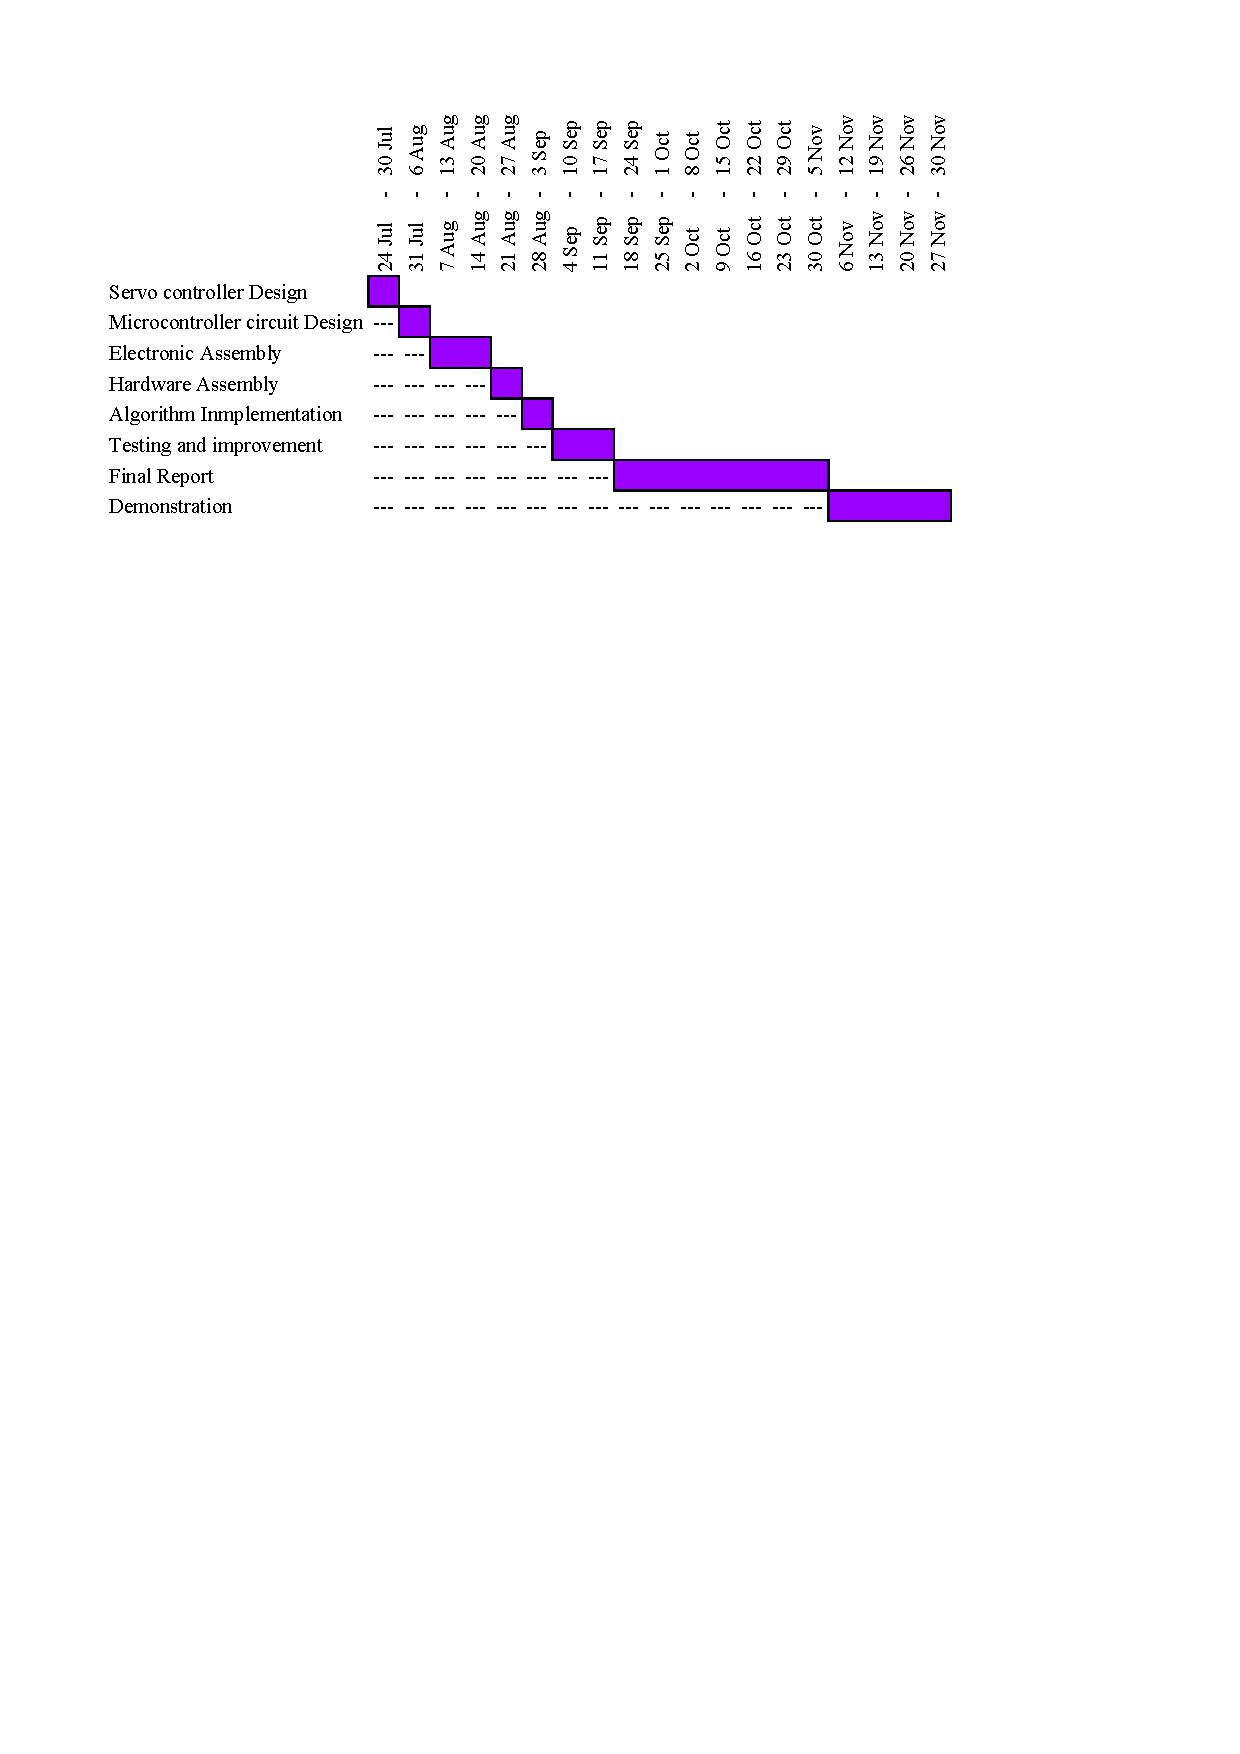
\includegraphics[clip, trim=1.5cm 21cm 1.5cm 1.5cm, width=1.00\textwidth]{pics/Gantt2.pdf}
    \caption{Gantt diagram for work to be completed}
    \label{fig:Gantt2}
\end{figure}
\FloatBarrier

%\vspace{30cm}

%\newpage

%% End of File.


%%
%%  Department of Electrical, Electronic and Computer Engineering.
%%  EPR400/2 Project Proposal - Section 4.
%%  Copyright (C) 2011-2017 University of Pretoria.
%%

\section{Specifications}

\subsection{Mission-critical system specifications}

\begin{center}
\begin{longtable}{|p{5cm}|p{5cm}|p{5cm}|}
\hline
  \textbf{SPECIFICATION (IN MEASURABLE TERMS)} &
  \textbf{ORIGIN OR MOTIVATION OF THIS SPECIFICATION} &
  \textbf{HOW WILL YOU CONFIRM THAT YOUR SYSTEM COMPLIES WITH
           THIS SPECIFICATION?}\\
\hline
   &
   &
   \\
\hline
   &
   &
   \\
\hline
   &
   &
   \\
\hline
\caption{Mission-critical system specification}
\end{longtable}
\end{center}

\subsection{Field conditions}

\begin{center}
\begin{longtable}{|p{7.5cm}|p{7.5cm}|}
\hline
  \textbf{REQUIREMENT} &
  \textbf{SPECIFICATION (IN MEASURABLE TERMS)} \\
\hline
   &
   \\
\hline
   &
   \\
\hline
   &
   \\
\hline
\caption{Field conditions}
\end{longtable}
\end{center}

\subsection{Functional unit specifications}

\begin{center}
\begin{longtable}{|p{7.5cm}|p{7.5cm}|}
\hline
  \textbf{SPECIFICATION} & \textbf{ORIGIN OR MOTIVATION} \\
\hline
   &
   \\
\hline
   &
   \\
\hline
\caption{Functional unit specifications}
\end{longtable}
\end{center}

\newpage

%% End of File.



%%
%%  Department of Electrical, Electronic and Computer Engineering.
%%  EPR400/2 Project Proposal - Section 5.
%%  Copyright (C) 2011-2017 University of Pretoria.
%%

\section*{5. Deliverables}
\addcontentsline{toc}{subsection}{5. Deliverables}

\subsection*{Technical deliverables}

\begin{center}
\begin{longtable}{|p{7cm}|p{3.5cm}|p{3.5cm}|}
\hline
\textbf{DELIVERABLE} & \textbf{DESIGNED AND IMPLEMENTED BY STUDENT} &
\textbf{OFF-THE-SHELF} \\
\hline  Microcontroller for control of the robot.
         &     & \multicolumn{1}{c|}{X}\\
\hline Control code for inverse kinematics and servo control.
         &   \multicolumn{1}{c|}{X}  &  \\
\hline Android application with a user interface for control of the robot.
         &   \multicolumn{1}{c|}{X}  &  \\
\hline Wireless module for communication between the smartphone interface and the robot
         &     &  \multicolumn{1}{c|}{X}\\
\hline Circuits implemented on PCB for interfacing all hardware with the microcontroller.
         &  \multicolumn{1}{c|}{X}   &  \\
\hline Servo motors for movement of the joints.
	&	&\multicolumn{1}{c|}{X}	\\
	\hline Robot body and legs.
	&	\multicolumn{1}{c|}{X}&	\\
	\hline Simulations on all implemented software and analogue design
	&	\multicolumn{1}{c|}{X}&	\\
\hline
\caption{Deliverables}
\end{longtable}
\end{center}

\subsection*{Demonstration at the examination}
\begin{enumerate}
\item The robot will be placed on a grid on the floor and the examiners will be shown that the robot is capable of holonomic movement.
\item The centre of the robot will be noted on the grid and the examiners will see that the robot is capable of rotating around its centre without translating.
\item The robot will execute a specific set of movements while the time to completion is being recorded.
\item Small obstacles will be placed in the way of the robot to make movement more challenging. This includes small blocks to step over as well as a change in surface such as sand.
\item The robot will repeat the set of movements over the obstacles while the time to completion is measured again.
\item The examiners will see that the robot is capable of moving with similar effort over various surfaces.
\end{enumerate}

\newpage

%% End of File.



\setcounter{subsection}{5}
\titleformat{\subsection}[frame]
{\fontsize{12pt}{14.4pt}\selectfont\bfseries} {} {5pt} {\thesubsection\quad}
\printbibliography[heading=subbibnumbered]
\end{refsection}